\ifdefined\DIPLOMA
    \section{Техническое задание}

    Спроектировать малый привод манипулятора, устанавливаемого на малом спутнике
    съёмки Земли (рис. \ref{sattelite_general_view}).
\else
    \subsection{Назначение и общий вид манипулятора}

    Целью данной курсовой работы ставится проектирование одного из двух
    приводов манипулятора, устанавливаемых на малых спутниках съемки Земли
    (рис. \ref{sattelite_general_view}).

    В данный момент манипуляторы подобного рода на спутниках широко востребованы
    в областях картографирования, планировки территорий, образовательных,
    разведывательных и военных целях, метеорологии и т.п.

    К подобным манипуляторам предъявляют высокие требования по точности,
    надежности, массе, габаритам.
\fi

Манипулятор входит в состав двухзвенного электроприводного механизма,
предназначенного для скоростного наведения оптических камер.
Задачей манипулятора является организация перенацеливания камеры с приведённым
моментом инерции $J_{oy} = 3 ~\text{кг} \cdot \text{м}^2$ в заданное положение.

\begin{figure}[h!]
    \centering
    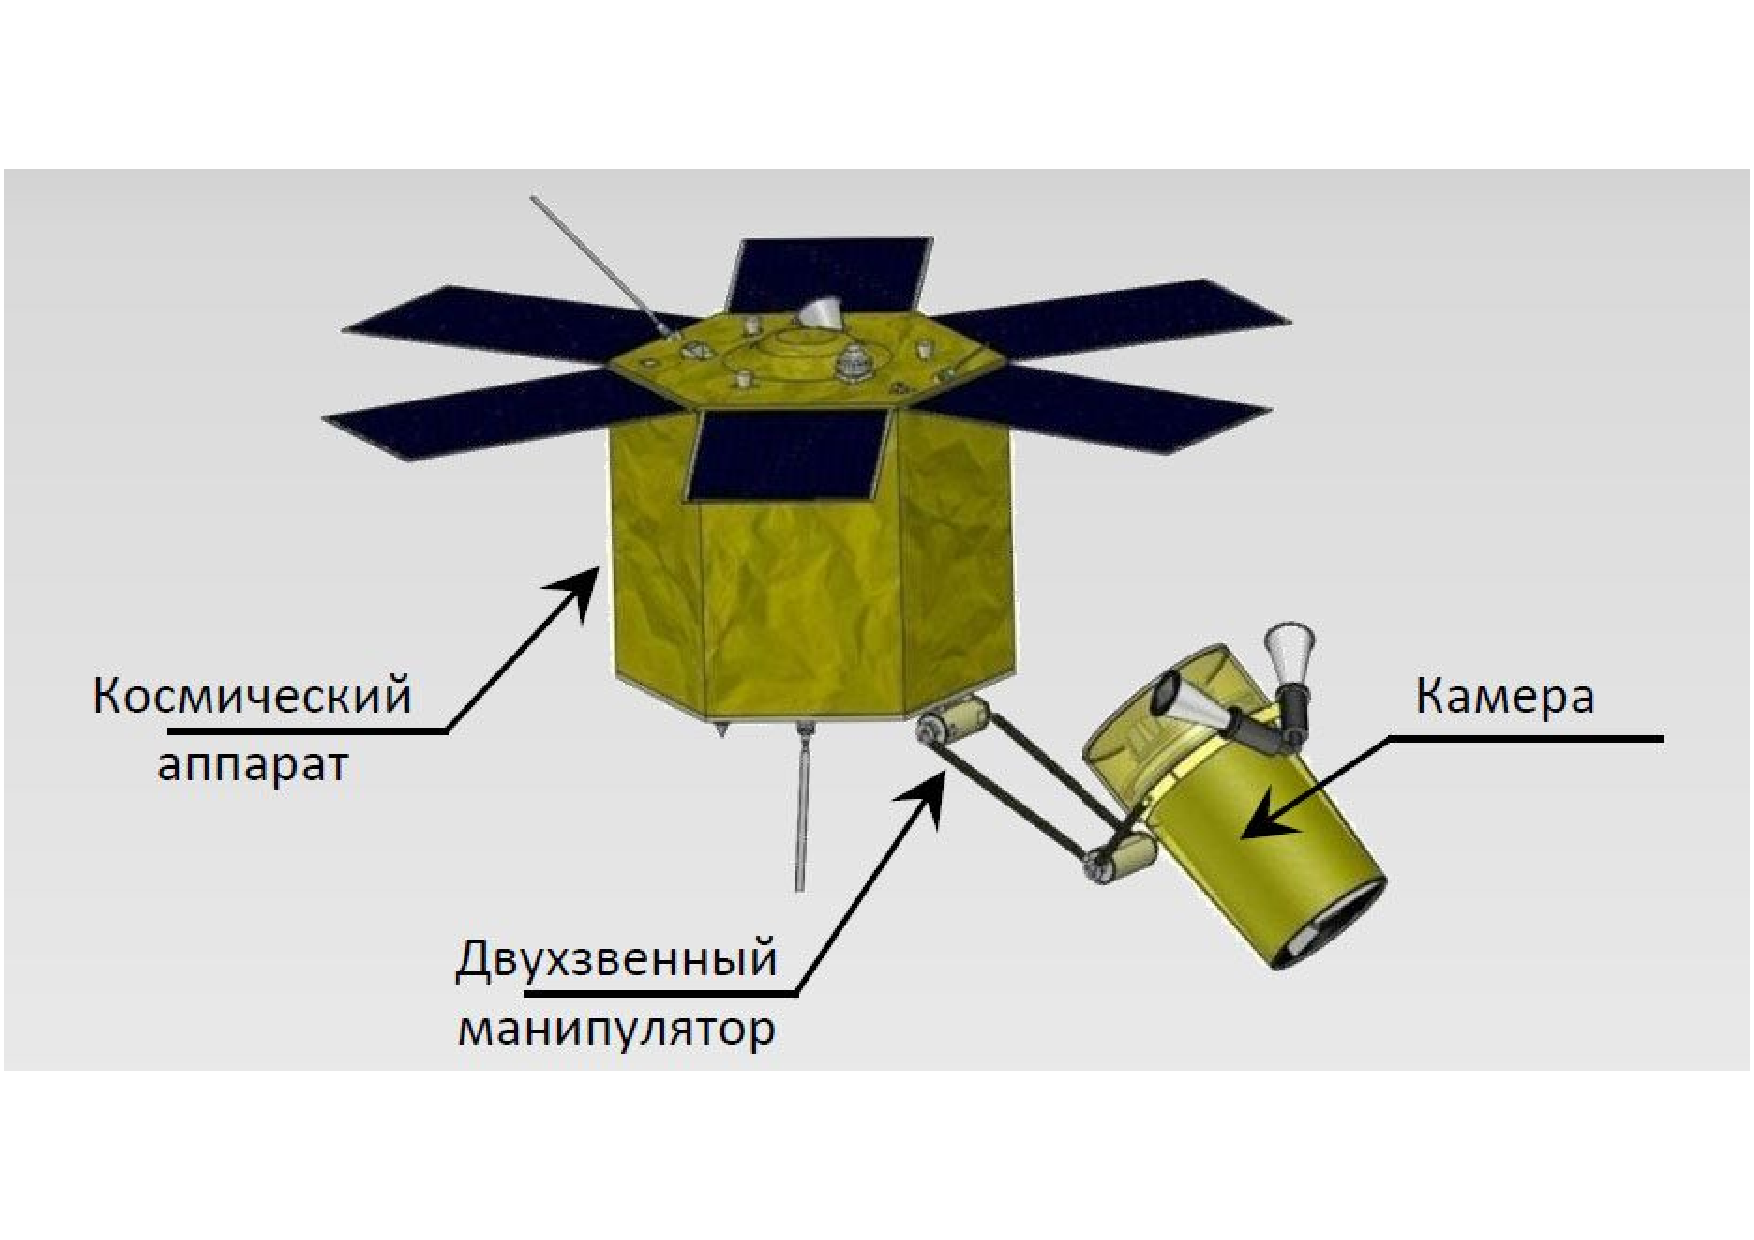
\includegraphics[width=\textwidth, keepaspectratio, clip=true, trim=3cm 3cm 3cm 3cm]
                    {./src/pictures/sattelite_3d_images/general_view}
    \caption{Манипулятор наведения камеры малого спутника Земли}
    \label{sattelite_general_view}
\end{figure}

Программные движения манипулятора осуществляются с электроприводных блоков,
обеспечивающего поворот камеры в одной плоскости (в плоскости перпендикулярной
вектору движения космического аппарата по орбите).

Точность позиционирования нагрузки $q_d \leq 1'$.

Максимальный диапазон углового перенацеливания камеры: $\beta_{max} = -45..+45^\circ$.
Привод должен обеспечивать режимы переброски удовлетворяющие следующим 3~-- м движениям:

\begin{enumerate}
    \item Перенацеливание камеры на $q = 20^\circ$ за $t_\textit{п} = 2  $ c
    \item Перенацеливание камеры на $q = 45^\circ$ за $t_\textit{п} = 3  $ c
    \item Перенацеливание камеры на $q = 90^\circ$ за $t_\textit{п} = 4.3$ c
\end{enumerate}

Ресурс привода должен быть не менее 30 тыс. часов.
